
\section*{1. The question has become more precise}\phantomsection\addcontentsline{toc}{section}{1. The question has become more precise}
The question "Does AI Help?" is reasonable, but it compresses several different questions. Does an assistant reduce the time required for a task? Does it improve the quality of the result? Does it allow a person to attempt work that would otherwise be infeasible? Does it improve a team's throughput or an organization's performance? Does it strengthen the human capacity needed to judge future results? Does it expand useful knowledge?


These questions have different units of analysis and different counterfactuals. A shorter drafting session can be a real benefit even if the organization has no additional demand for the resulting documents. A successful prototype may be valuable because it enables an experiment, while remaining unsuitable for production. A correct scientific calculation can save weeks of work without resolving an important scientific uncertainty. A student may produce excellent work while learning less than another student who struggled through the same problem.


The literature has moved from demonstrations of task acceleration toward these more demanding distinctions. Our assessment is that the evidence supports substantial, already realized assistance in particular settings. It does not support a single percentage improvement for intellectual work as a whole. The defensible claim is conditional: AI helps when its capabilities fit the task, its outputs can be evaluated with sufficient credibility, and its contribution survives the constraints of the surrounding process.


This condition does not restrict AI to easy problems. Difficult mathematics, complex empirical software, and cross-disciplinary research can benefit from AI precisely because generating and exploring candidate solutions is costly. The relevant requirement is a credible validation process whose cost and residual uncertainty are acceptable. We therefore examine both acceleration of existing work and expansion of work that becomes feasible.



\subsection*{Companion reviews and reference works}\phantomsection\addcontentsline{toc}{subsection}{Companion reviews and reference works}
This review is not the first synthesis of AI's effects. OECD's 2025 experimental-evidence review covers productivity, innovation and entrepreneurship; ILO's 2026 brief connects task-level results with employment and work organization. Stanford's 2026 AI Index supplies a broader reference map across capability, economy, science and education. These are valuable entry points, but draw in part on the same underlying evidence reviewed here. They are not additional independent replications. [\hyperlink{ref-oecdproductivity2025}{1}, \hyperlink{ref-iloreview2026}{2}, \hyperlink{ref-aiindex2026}{3}]


For software, Mohamed and colleagues map 39 studies, while Wittig and colleagues examine the fragmented operationalization of productivity across 187 markers. Maier and colleagues provide a quantitative synthesis rather than a universal percentage gain: their programming-productivity estimate is a standardized effect, combining heterogeneous outcomes and settings. [\hyperlink{ref-ref-59e035c44a}{4}, \hyperlink{ref-wittig2026}{5}, \hyperlink{ref-maier2026}{6}]


For learning, OECD's education outlook, a programming-education review, and recent meta-analyses offer complementary but sometimes conflicting results. For science, the Agentic Science survey provides a taxonomy of capabilities and workflows, not proof of dependable autonomous discovery. Our distinctive contribution is to connect these domains through the distinction between production, verification, integration, use and value, while preserving differences in design and evidentiary strength. [\hyperlink{ref-oecdeducation2026}{7}, \hyperlink{ref-ref-e71e370e4c}{8}, \hyperlink{ref-agenticsurvey2025}{9}]



\section*{2. How the evidence developed, 2021-2026}\phantomsection\addcontentsline{toc}{section}{2. How the evidence developed, 2021-2026}

\subsection*{2021-2022: specialized capability and measurement foundations}\phantomsection\addcontentsline{toc}{subsection}{2021-2022: specialized capability and measurement foundations}
Two foundations predate the current chatbot debate. AlphaFold established that a specialized AI system could transform a scientifically important prediction task. It also illustrates why prediction and downstream scientific or therapeutic impact must be assessed separately. In software engineering, the SPACE framework formalized an older lesson: productivity includes satisfaction, performance, activity, collaboration, and flow, and cannot be reduced to one activity metric. These foundations remain useful even as the technology changes. [\hyperlink{ref-alphafold2021}{10}, \hyperlink{ref-space2021}{11}]



\subsection*{2023: early experimental gains and an uneven frontier}\phantomsection\addcontentsline{toc}{subsection}{2023: early experimental gains and an uneven frontier}
The first wave of broadly accessible generative tools produced persuasive evidence of assistance. Noy and Zhang's writing experiment reported shorter completion times and better assessed artifacts. The Copilot experiment reported a large time reduction on an isolated programming task. Dell'Acqua and colleagues' consultant experiment introduced an especially important complication: an assistant can improve performance on one task while encouraging errors on another task that appears comparable to its user. [\hyperlink{ref-noy2023}{12}, \hyperlink{ref-peng2023}{13}, \hyperlink{ref-dellacqua2023}{14}]


The intellectual shift was from "the model can produce this" to "access to the model changes human performance under specified conditions." It was also becoming clear that model fluency does not reliably indicate whether a task lies within its capabilities. In December 2023, FunSearch provided a different kind of demonstration: language-model proposals combined with systematic evaluation could improve mathematical constructions and algorithmic heuristics. [\hyperlink{ref-funsearch2023}{15}]



\subsection*{2024-2025: broader deployment, verification, and conflicting outcomes}\phantomsection\addcontentsline{toc}{subsection}{2024-2025: broader deployment, verification, and conflicting outcomes}
Evidence broadened beyond isolated tasks. Google's experiment investigated an enterprise-grade engineering task; larger workplace experiments examined access to coding assistance; the published customer-support study measured real operational throughput. At the same time, DORA's organizational work, code-quality studies, and conceptual research on scientific understanding questioned whether local production gains were sufficient evidence of wider benefit. [\hyperlink{ref-paradis2024}{16}, \hyperlink{ref-cui2025}{17}, \hyperlink{ref-brynjolfsson2025}{18}, \hyperlink{ref-dora2024}{19}, \hyperlink{ref-messeri2024}{20}]


METR's early-2025 maintainer experiment became a useful counterexample to universal acceleration. It did not show that AI was generally unhelpful. It showed that an apparently promising tool could slow a particular expert workflow, and that perceived speedup could disagree with measured task time. Education research increasingly distinguished performance with assistance from assessment after assistance was removed. [\hyperlink{ref-metr2025}{21}, \hyperlink{ref-bastani2025}{22}]



\subsection*{2026: agents, downstream outcomes, and the full research loop}\phantomsection\addcontentsline{toc}{subsection}{2026: agents, downstream outcomes, and the full research loop}
The next wave of evidence studies agents that act across repositories, run experiments, and continue work over extended periods. The questions become more organizational and epistemic: does increased code activity reach releases and users; does the learner retain understanding; can the agent distinguish improvement from measurement noise; and can a research result survive independent checking? [\hyperlink{ref-demirer2026}{23}, \hyperlink{ref-chenstratton2026}{24}, \hyperlink{ref-bergh2026}{25}, \hyperlink{ref-innovationeval2026}{26}]


Changing technology also changes measurement. METR's follow-up describes how increasing attachment to AI affects participation, task selection, and time accounting. A frozen experimental result can remain valid for its original setting while becoming a poor estimate of current tools. Conversely, a new model release is not itself evidence that all earlier organizational constraints have disappeared. [\hyperlink{ref-metr2026update}{27}]


The chronology is not a sequence in which optimism is simply replaced by skepticism. It is a progressive expansion of the outcome being evaluated. Early gains remain meaningful; subsequent evidence explains why they must be interpreted within larger processes.



\section*{3. What "how much" can legitimately mean}\phantomsection\addcontentsline{toc}{section}{3. What "how much" can legitimately mean}
Four distinctions organize this review. First, \textbf{capability} is what a system can accomplish under an evaluation protocol. Second, \textbf{assistance} is the effect of a person having access to the system. Third, \textbf{process performance} concerns the output of a workflow or organization. Fourth, \textbf{consequential value} concerns whether the output is used, improves decisions, advances knowledge, or creates benefits relative to its total cost.


Randomized experiments are especially informative about the effect of access in the tested population, but their conclusions may not transfer to other tasks or future models. Observational event studies can cover actual work at scale but rely on assumptions about adoption and comparison groups. Surveys capture experience, intentions, and perceived benefits; they do not independently measure the counterfactual. Benchmarks evaluate defined capabilities, often under unusually favorable instrumentation. Case studies reveal mechanisms and possible uses but cannot establish prevalence. Peer review improves scrutiny without changing the fundamental identification strategy of a study.


Selected findings make the diversity concrete:



{\footnotesize\setlength{\tabcolsep}{3pt}\renewcommand{\arraystretch}{1.25}
\begin{longtable}{>{\raggedright\arraybackslash}p{0.230\textwidth}>{\raggedright\arraybackslash}p{0.230\textwidth}>{\raggedright\arraybackslash}p{0.230\textwidth}>{\raggedright\arraybackslash}p{0.230\textwidth}}\toprule
Setting and source & Outcome measured & Reported result & Interpretation boundary \\\midrule\endhead
Professional writing, 2023 [\hyperlink{ref-noy2023}{12}] & Task time; assessed artifact quality & 40\% less time; 18\% higher quality & Bounded writing tasks, not firm productivity \\
Customer support, journal version 2025 [\hyperlink{ref-brynjolfsson2025}{18}] & Issues resolved per hour & 15\% average increase & Embedded workflow in one business setting \\
Enterprise coding task, 2024 [\hyperlink{ref-paradis2024}{16}] & Task time & About 21\% reduction & Wide uncertainty; 96 engineers \\
Three coding field experiments [\hyperlink{ref-cui2025}{17}] & Completed tasks & About 26\% increase & Different task measures and organizations \\
Expert maintainers, early 2025 [\hyperlink{ref-metr2025}{21}] & Time on familiar-repository work & 19\% longer & Small expert population; early-2025 tools \\
Firm adoption of coding agents [\hyperlink{ref-chenstratton2026}{24}] & Code activity; PR-to-merge time & More activity; longer review cycle & No proportional increase in issue/epic output \\
Programming students, 2026 [\hyperlink{ref-bergh2026}{25}] & Assisted coding; subsequent recall & Better code; lower recall & Short experiment; not a long-run skill estimate \\
\bottomrule\end{longtable}}
These numbers should not be averaged or ranked as competing estimates of one quantity. A time reduction and a throughput increase have different denominators. Cumulative event-study effects also differ from instantaneous changes. The tables in this review are evidence comparisons, not a meta-analysis.


The SPACE framework and recent mixed-methods research support broader measurement that includes ownership, expertise, and the distribution of effort. They are useful because an organization can improve an easily counted activity while burdening work that is harder to see. [\hyperlink{ref-space2021}{11}, \hyperlink{ref-chen2026}{28}, \hyperlink{ref-afroz2025}{29}]



\section*{4. Where assistance is already demonstrated}\phantomsection\addcontentsline{toc}{section}{4. Where assistance is already demonstrated}

\subsection*{Bounded writing and operational support}\phantomsection\addcontentsline{toc}{subsection}{Bounded writing and operational support}
Writing assistance is among the clearest early examples of a measurable task benefit. Noy and Zhang studied occupational writing with randomized access, rather than relying solely on users' impressions. That result supports assistance for the tested work; it does not establish that all generated communication is useful or that persuasive writing is factually correct. [\hyperlink{ref-noy2023}{12}]


The customer-support study adds an operational setting. Its staggered rollout among 5,172 agents yields a published 15\% average increase in issues resolved per hour. Gains were heterogeneous: less experienced and lower-skilled workers improved speed and quality, while the most experienced and highest-skilled workers had small speed gains and small quality declines. The authors also report evidence consistent with worker learning, including performance during tool outages. These findings show that assistance can reach a consequential workflow metric without benefiting every group on every outcome. The quasi-experimental design depends on identification assumptions; transfer to unfamiliar domains remains an empirical question. [\hyperlink{ref-brynjolfsson2025}{18}]



\subsection*{Programming within a suitable context}\phantomsection\addcontentsline{toc}{subsection}{Programming within a suitable context}
The coding experiments provide credible reasons to use assistance, especially where users can quickly integrate suggestions into a well-scoped task. Microsoft's CLI-agent rollout also associates agent adoption with more merged PRs over several months. These are operationally meaningful effects, although the latter outcome remains a proxy for value. [\hyperlink{ref-cui2025}{17}, \hyperlink{ref-murphyhill2026}{30}]


The maintainer counterexample is a measured cost, not merely a caveat to the positive experiments: METR's randomized early-2025 study found that 16 experienced maintainers took 19\% longer across 246 tasks when allowed AI tools. Participants nevertheless believed they had become faster. In mature repositories, interpreting implicit conventions and checking changes can outweigh saved implementation time. The mechanism is plausible, not universal; the small expert sample and tool vintage limit transfer. The follow-up changes the current measurement problem, but does not erase the original slowdown. [\hyperlink{ref-metr2025}{21}, \hyperlink{ref-metr2026update}{27}]



\subsection*{Removing a specific scientific constraint}\phantomsection\addcontentsline{toc}{subsection}{Removing a specific scientific constraint}
Specialized prediction and computational search offer a third category of demonstrated benefit. They do not need to imitate an entire human scientist to be valuable. If a system improves an important intermediate step, it can change the set of experiments or analyses researchers can attempt. The downstream assessment of AlphaFold is particularly informative: it describes complementary use with experimental biology and expanded basic research, while finding no comparable early shift in applied drug-development targeting. [\hyperlink{ref-alphafoldimpact2026}{31}]


Our interpretation is that the most credible benefits so far often arise when AI is placed within a functioning process, rather than asked to define and replace the whole process. This is a synthesis of the cases, not a claim that narrow use is the only future possibility.



\section*{5. From more code to better engineering}\phantomsection\addcontentsline{toc}{section}{5. From more code to better engineering}
The strongest recent engineering distinction concerns the production hierarchy. In the September revision of \emph{Writing Code vs. Shipping Code}, Demirer, Musolff, and Liyuan Yang analyze more than 500,000 developers. Their large cumulative effects on commits attenuate substantially for projects and releases, and the marketplace analysis does not show increased total application usage. This supports attention to downstream constraints rather than treating commits as interchangeable with delivered value. [\hyperlink{ref-demirer2026}{23}]


Chen and Stratton examine a different, firm-centered dataset: 718 organizations using Jellyfish. They find increased code activity after coding-agent adoption and a longer review cycle, with limited pass-through to resolved issues and epics. Their statistically insignificant output estimates do not prove exactly zero benefit; their confidence bounds are more informative than the popular headline. PR-to-merge time includes waiting, coordination, and revision as well as active review. [\hyperlink{ref-chenstratton2026}{24}]


In the August version, agent adoption increases code-line output by about 30\%, whereas the estimates rule out an increase above 12\% of the baseline mean in their firm-level output measures. That is evidence against proportional pass-through, not a finding of exactly no software benefit. Conversely, He and colleagues' single-enterprise panel reaches 2.09 times baseline merged PRs per developer while reviewer load roughly doubles. Its nonrandom adoption, newer-code concentration and stable merge/revert rates do not establish equivalent gains in useful releases or defect-free production. These studies should not be averaged into one engineering percentage. [\hyperlink{ref-chenstratton2026}{24}, \hyperlink{ref-hemandate2026}{32}]


Vendor reports from Faros and GitClear add useful signals about larger changes, duplication, review pressure, and maintenance. Their large samples do not remove selection or calendar-time confounding. DORA supplies a broader organizational interpretation in which AI amplifies existing conditions. These accounts should be compared at the level of their measured outcomes, not treated as rival universal theories resolved by sample size. [\hyperlink{ref-faros2026}{33}, \hyperlink{ref-gitclear2025}{34}, \hyperlink{ref-dora2025}{35}, \hyperlink{ref-doratensions2026}{36}]


A contrasting repository study by Hamza, Siemon and Awan compares 669 developer-repository pairs with 228 control pairs. It finds longer PR descriptions and small testing-related associations after visible agent participation, but the review changes seen in before/after comparisons do not remain significant relative to controls. This cautions against attributing every adverse review trend to AI. It does not show that agents improve delivered software: adoption is nonrandom, control periods use repository-specific median dates, and description length and test-file changes are imperfect proxies for quality. A nonsignificant review contrast also does not establish equivalence. [\hyperlink{ref-hamza2026}{37}]


Quality itself is multidimensional. Studies of generated code identify differing defect profiles, while static analysis shows that passing tests is an incomplete indicator of security or maintainability. Production C++ analysis extends the question to review effort and execution-resource consumption. An intervention that reduces development time can still increase the lifetime cost of the resulting software. [\hyperlink{ref-cotroneo2025}{38}, \hyperlink{ref-sabra2025}{39}, \hyperlink{ref-tran2026}{40}]


Evaluation is accordingly becoming longitudinal. SWE-CI tests successive repository changes, and coverage research asks whether changed lines are exercised. Coverage remains weaker than a test that asserts the right behavior. Iterative infrastructure repair also illustrates a measurement hazard: a best-so-far curve cannot reveal every regression between attempts, and the estimated regression rate depends strongly on how validator results are mapped to changes. [\hyperlink{ref-sweci2026}{41}, \hyperlink{ref-coverage2026}{42}, \hyperlink{ref-iac2026}{43}]


Formal verification offers stronger assurance under explicit specifications. Vero's joint implementation and proof tasks demonstrate progress and substantial remaining limits. A checker certifies a relationship between a program and a formal specification; it cannot independently decide whether that specification represents the user's intentions or the relevant real-world conditions. [\hyperlink{ref-vero2026}{44}]



\subsection*{Contribution boundaries and the costs borne by others}\phantomsection\addcontentsline{toc}{subsection}{Contribution boundaries and the costs borne by others}
Technical capability does not imply an entitlement to submit generated work. QEMU defaults to declining contributions containing or derived from AI-generated content because of provenance and Developer Certificate of Origin concerns. Research or debugging assistance is permitted if generated output is not submitted. The policy allows proposals for specific exceptions through project discussion, without waiving human certification; the inspected text lists no approved exceptions. Its introducing repository commit is dated 24 June 2025. These are project judgments, not our legal conclusions or productivity findings. [\hyperlink{ref-qemupolicy2026}{45}]


Other prominent restrictions differ in scope. GIMP prohibits generative-AI contributions in code, images and text. Redox rejects LLM-generated submissions, including issues and merge-request descriptions. Zig's designated development spaces additionally prohibit LLM-assisted editing, translation, shared brainstorming results and bug finding; independent Zig communities are outside those rules. NetBSD presumes generated code tainted but explicitly allows prior written core approval. It is therefore inaccurate to describe all four as identical, exceptionless bans on every use of AI. [\hyperlink{ref-gimppolicy2026}{46}, \hyperlink{ref-redoxpolicy2026}{47}, \hyperlink{ref-zigpolicy2026}{48}, \hyperlink{ref-netbsdpolicy2024}{49}]


Linux provides a contrasting conditional framework: tool-generated contributions require human understanding, transparent provenance, testing and responsibility for sign-off. Individual maintainers retain discretion to reject them or demand additional scrutiny. AI-assistant guidance adds attribution and reproduction requirements. This is neither universal rejection nor automatic acceptance. [\hyperlink{ref-linuxgenerated2026}{50}, \hyperlink{ref-linuxassistants2026}{51}]


A concrete favorable episode is Torvalds's October 2026 associative-array work. Phoronix quotes his account of LLM-assisted understanding and refactoring, followed by user-space test-harness execution that confirmed a reported bug and found three additional longstanding bugs. The article reports the changes as not yet merged to master. This illustrates assisted comprehension coupled with executable checks, not proof that the LLM independently discovered every bug or improved kernel-wide productivity. [\hyperlink{ref-torvaldsassoc2026}{52}]


Policy disagreement can also change project boundaries. Asahi broadly forbids generative-AI tooling for material contributions, citing ethical concerns and clean-room risks. Gravity's own FAQ says it initially forked from Asahi over LLM-policy differences. Gravity permits and encourages responsible LLM use, but requires disclosure, human accountability and demonstrable clean-room provenance, and prohibits laundering proprietary implementation details through a model. The contrast is genuine; neither approach's engineering superiority follows from its stated policy. [\hyperlink{ref-asahipolicy2026}{53}, \hyperlink{ref-gravityabout2026}{54}, \hyperlink{ref-gravitypolicy2026}{55}]


Ghostty illustrates a different policy: responsible AI-written text and code are allowed, with disclosure and human understanding required; generated media are prohibited. First-time contributors need a maintainer's vouch, and unvouched PRs are closed. The project explicitly welcomes AI while protecting reviewers from low-quality submissions. Calling this a blanket AI-code ban would be misleading. These policies document who bears validation costs and controls participation, not how common such views are across open source. [\hyperlink{ref-ghosttypolicy2026}{56}, \hyperlink{ref-ghosttycontribution2026}{57}]


Broader policy evidence prevents prominent bans from becoming a misleading picture of the whole community. Hora, Robbes and Zacchiroli identify 281 policies in a September 2026 study: 83.3\% permit or encourage AI code contributions, while 14.9\% forbid them. The denominator is identified policies in popular active repositories and selected prominent projects, not all open source. This expanded study is related to the authors' earlier work, not an independent replication; changed sampling and detection also prevent interpreting their different percentages as a clean time trend. Documented rules do not establish compliance, policy effectiveness or net productivity. [\hyperlink{ref-horapolicies2026}{58}]


The managerial implication is to evaluate the whole change lifecycle. Useful measures include elapsed time to acceptance, rework, defect escape, security, resource use, and adoption of the delivered capability. The broader question is whether a team obtains more dependable useful functionality for its total effort and cost.



\section*{6. Assisted performance and human development}\phantomsection\addcontentsline{toc}{section}{6. Assisted performance and human development}
For a professional completing a task, outsourcing intermediate work may be rational. For a learner, that intermediate work can be the mechanism through which competence develops. The same intervention can therefore help immediate performance and weaken the preparation needed for future supervision.


Bastani and colleagues' mathematics trial distinguishes practice with AI from later unaided performance, and shows that instructional guardrails matter. Shen and Tamkin's programming-library experiments similarly examine conceptual understanding and debugging rather than just the delivered artifact. These studies support concern about unstructured delegation, while remaining specific to their subjects, participants, and implementations. [\hyperlink{ref-bastani2025}{22}, \hyperlink{ref-shen2026}{59}]


Poulidis and the Bastanis isolate assistance design in chess training. Both randomized groups receive automatic engine tips; one can additionally request answer-revealing help. Among 216 completers from 306 recruits, that additional access produces smaller gains on later unaided tests after 12 weeks of training. The frequently quoted 30\% versus 64\% refers to improvement in bounded test-game scores, not a percentage of underlying competence. Attrition and assumption-dependent mediation deserve scrutiny. The intervention uses Stockfish rather than an LLM, and has no randomized no-AI arm: it supports a warning about unrestricted solutions during practice, not a verdict against all AI tutoring. [\hyperlink{ref-ref-283d4e8368}{60}]


The September 2026 programming experiment by Bergh and colleagues supplies an unusually useful distinction. Students with ChatGPT produced stronger code but had lower recall immediately and after 48 hours. The study did not detect a significant difference in the rate of forgetting across that interval. The evidence concerns what was learned or encoded during the task, not a demonstrated acceleration of memory decay. [\hyperlink{ref-bergh2026}{25}]


Martin-Lopez and colleagues' crossover experiment shows the trade-off within one study: 69 participants complete substantially more of their tasks with AI, but median correct answers about their code fall from 100\% to 87.5\%, a 12.5-percentage-point difference. Only 14 participants were professionals. This is an immediate comprehension measure, not evidence of irreversible deskilling; nevertheless, the loss is an outcome in its own right, not something that better-looking code cancels out. [\hyperlink{ref-ownership2026}{61}]


Evidence is not uniformly negative. Lepp's observational course study finds no significant assessment differences among AI-interaction profiles. That finding neither proves equivalence nor establishes that the design of teaching is irrelevant. It indicates that broad categories of self-directed use may predict feelings about learning more readily than measured assessment. Wang's feedback framework proposes a more designed form of assistance, but retrospective prediction and message-quality checks still require prospective learning validation. [\hyperlink{ref-lepp2026}{62}, \hyperlink{ref-wang2026}{63}]


The synthesis literature does not resolve this into one verdict. Wu and colleagues report a positive learning estimate across 35 studies from 2022-2024. Boolzen and colleagues' newer STEM synthesis finds extreme heterogeneity and a mean close to zero after Bayesian publication-bias adjustment. Conversely, September v5 of the living mathematics meta-analysis reports a positive estimate across 34 studies. Different populations, outcomes, eligibility rules and statistical assumptions can change the answer; neither a favorable mean nor a bias-adjusted null applies to every instructional design. Overlapping trials must not be counted repeatedly. [\hyperlink{ref-wulearning2026}{64}, \hyperlink{ref-boolzen2026}{65}, \hyperlink{ref-llamalima2026}{66}]


Maier and colleagues' programming meta-analysis likewise separates a positive productivity estimate from a learning estimate whose confidence interval includes zero. That is uncertainty about learning benefit, not proof of no effect or permanent deskilling. Standardized effects cannot be translated directly into percentages of time saved. [\hyperlink{ref-maier2026}{6}]


A second developmental question concerns working experts. Longitudinal survey work describes a shift from creation toward supervisory engineering; a small field study relates cognitive load to task context and AI use. Such evidence is relevant to the experience and distribution of work, but cannot on its own establish neurological harm, permanent skill loss, or an overall causal reduction in effort. [\hyperlink{ref-vella2026}{67}, \hyperlink{ref-brand2026}{68}]


Hicks, Lee and Foster-Marks add the psychological and organizational dimension. Their 3,267-person observational survey relates competitive and innate-brilliance beliefs to reported AI-related identity threat, while learning culture and belonging accompany more favorable reported experiences. This is not causal evidence that culture interventions increase productivity, and its performance measures are self-reported. Neither identity threat nor reluctance to adopt AI makes concerns about reliability, employment or provenance unfounded. A responsible interpretation takes those concerns seriously rather than diagnosing resistance as a defect in the worker. [\hyperlink{ref-ref-47ac0a3015}{69}]


Our interpretation is that the relevant educational aim is an accountable relationship to assisted work. Learners should be able to explain the result, recover essential reasoning, detect consequential errors, and transfer knowledge to a new task. Institutions need evidence about those abilities, especially when polished artifacts cease to be reliable evidence of independent understanding. The optimal balance between assisted practice and unaided work remains a subject for intervention research.



\section*{7. Scientific discovery: prediction, search, and judgment}\phantomsection\addcontentsline{toc}{section}{7. Scientific discovery: prediction, search, and judgment}
AI's scientific contribution spans several distinct activities: organizing literature, writing empirical software, generating hypotheses, finding algorithms, establishing formal proofs, and conducting a research process. Success in one is informative but insufficient to establish success in all.


ERA demonstrates evaluator-guided search over empirical software. Co-Scientist and Robin connect generated hypotheses or analyses with selected expert and experimental validation. The AI Scientist explores a more extended ML-research workflow, including evaluation of generated work by workshop review. Each represents a meaningful expansion of the toolchain. Their scientific credibility depends on the particular validation process, the selection of cases, and the contribution of human investigators. [\hyperlink{ref-era2026}{70}, \hyperlink{ref-coscientist2026}{71}, \hyperlink{ref-robin2026}{72}, \hyperlink{ref-aiscientist2026}{73}]


Formal mathematics and algorithm search illustrate why difficult problems can be suitable for AI. AlphaProof benefits from a machine-checkable formal environment. AlphaEvolve and DiscoRL use feedback to explore algorithms or learning rules. These systems provide stronger evidence than a fluent narrative asserting a discovery, because an external procedure can reject many unsuccessful proposals. The meaning of the result still depends on the problem formulation and the domain of transfer. [\hyperlink{ref-alphaproof2025}{74}, \hyperlink{ref-alphaevolve2025}{75}, \hyperlink{ref-discorl2025}{76}]


The value can also lie in connecting established methods that humans have not economically brought together. Schwartz's October account of BootLoops describes cross-disciplinary quantitative work in which experts helped distinguish a technically interesting computation from a scientifically important result. The account is a selected case study, with disclosed affiliation and ongoing validation, rather than a controlled estimate of research productivity. It nevertheless offers a useful mechanism for making previously impractical investigations possible. [\hyperlink{ref-schwartz2026}{77}]


This distinction changes the evaluation question. It is not enough to count correct calculations or generated manuscripts. One must ask whether the result is new, whether its interpretation is sound, whether the underlying evidence supports it, and whether it matters to the field. Scientific importance is partly a collective judgment informed by replication, explanation, and the problems researchers need to resolve.


Messeri and Crockett's perspective warns of illusions of understanding and scientific monocultures. Hao and colleagues' large historical analysis supplies a related but different observational result: individual advantages associated with AI use can coexist with a narrower collective distribution of research. That study covers broader historical AI than recent LLM assistants, and should not be used as a causal estimate of chatbot-induced contraction. [\hyperlink{ref-messeri2024}{20}, \hyperlink{ref-hao2026}{78}]


The evidence therefore supports optimism about new computational reach and caution about equating local scientific output with the health of scientific inquiry. Systems can make difficult work more feasible while concentrating attention on questions with abundant data and convenient evaluators. Maintaining diversity of problems and methods is part of assessing the benefit.



\subsection*{Mathematical capability, understanding and consent}\phantomsection\addcontentsline{toc}{subsection}{Mathematical capability, understanding and consent}
The June \emph{Leiden Declaration on Artificial Intelligence and Mathematics}, endorsed by the International Mathematical Union, supplies an earlier governance framework: disclose tools, retain human responsibility for correctness and authorship, credit prior work, support rigorous review, and protect research autonomy and open science. It recognizes AI's potential rather than proposing a blanket prohibition. These are community recommendations, not measured effects or evidence of unanimous agreement. [\hyperlink{ref-leiden2026}{79}]


Tao's 2026 ICM essay separates the arrival of capable mathematical tools from the question of what mathematics values. His October \emph{Math 2.0} lecture recognizes powerful problem solving while proposing a broader aim: use AI to improve exposition, research networks, formal libraries and human understanding, not merely accumulate solutions. This is a substantive expert agenda, not measured proof that automated mathematics is harmful. Klowden and Tao's earlier philosophical essay supplies the human-centered framing. [\hyperlink{ref-taoicm2026}{80}, \hyperlink{ref-taomath2026}{81}, \hyperlink{ref-klowdentao2026}{82}]


Opposition is not confined to doubtful capability. The September declaration \emph{A Severe Misalignment of AI in Mathematics}, initiated by 25 Fields medallists, recognizes advances but contests the incentives and effects of problem-count optimization. In October, the Association for Human Mathematics rejects OpenAI's mass-release model and calls for mathematicians to discontinue collaboration with the company. These are explicit, consequential positions, not population surveys or technical disproofs. They deserve representation without being described as the unanimous opinion of mathematics. Tao's AI-assisted, personally reviewed living summary also shows that criticism of particular practices can coexist with active AI use. [\hyperlink{ref-mathmisalignment2026}{83}, \hyperlink{ref-ahm2026}{84}, \hyperlink{ref-taoliving2026}{85}]



\subsection*{Navier-Stokes: what a proof certificate does and does not settle}\phantomsection\addcontentsline{toc}{subsection}{Navier-Stokes: what a proof certificate does and does not settle}
On 8 September, OpenAI announced a resolution of the Navier-Stokes Millennium problem and released a written manuscript and Lean artifacts. The claim concerns smooth forced breakdown alternatives, not a demonstration of all unforced fluid behavior. We inspected the stated theorem and outline, not every lemma or the running proof kernels. Clay's 11 September statement welcomes the apparent resolution while retaining its deliberate evaluation process; it is not a prize award. [\hyperlink{ref-openainavier2026}{86}, \hyperlink{ref-openainavierpaper2026}{87}, \hyperlink{ref-openainaviercode2026}{88}, \hyperlink{ref-claynavier2026}{89}]


Bastounis, Circelli and Hansen's 6 October preprint reports differences between the written argument and Lean lemmas, including derivative requirements. Its central warning is that a checked formal argument need not faithfully reproduce an accompanying natural-language argument. The authors explicitly do not adjudicate the correctness of the written proof. The theoretical worst-case result does not make every practical translation impossible. Nor does a discrepancy alone establish that the formal theorem is false. We retain the developer claim and the critique as distinct validation questions that this review does not resolve, rather than independently certifying or rejecting the claimed solution. [\hyperlink{ref-naviertranslation2026}{90}]


Hales provides a complementary technical account: kernel validity, statement fidelity, independent checking and readable exposition are different assurance layers. Lean's maintainer documents a positive AI contribution to finding and repairing soundness bugs, while treating adversarial proof artifacts as a genuine risk. Together these accounts show why formal mathematics is promising without being verification-free. [\hyperlink{ref-hales2026}{91}, \hyperlink{ref-demourakernel2026}{92}]



\section*{8. Can AI improve the next generation of AI?}\phantomsection\addcontentsline{toc}{section}{8. Can AI improve the next generation of AI?}
AI already contributes to components of AI development, but several layers should be distinguished. Optimizing a kernel, improving training data, proposing a learning rule, changing an agent's tools, and building a new foundation model are different activities. They require different evidence of transfer and autonomy.


Darwin Godel Machine and more recent harness-evolution work demonstrate a route through changes to agent software. A frozen model can power an improving system when the surrounding prompts, tools, memory, and control flow change. Tool-architecture experiments reinforce this point: agent behavior and costs depend on the interface through which capabilities are exposed, not only on the underlying model. [\hyperlink{ref-dgm2025}{93}, \hyperlink{ref-darwinx2026}{94}, \hyperlink{ref-interfaces2026}{95}]


InnovationEval asks a harder question about independent algorithmic research. The October report evaluates whether agents can develop a post-training method comparable to a withheld human innovation. The tested configurations make limited progress, and the report identifies misleading selection of favorable runs. Its interpretation is bounded by one task, few runs, scope judgments, and successor-model contamination. [\hyperlink{ref-innovationeval2026}{26}]


ResearchGym also distinguishes occasional strong results from reliable long research workflows. A single success can establish possibility without making the process dependable. Conversely, a failed benchmark run cannot establish that no useful AI-assisted research exists. [\hyperlink{ref-researchgym2026}{96}]


Automated alignment research offers a positive contrast under another protocol: agents improve metrics for defined unwanted behaviors, with selected held-out and transfer evaluations. The human comparison does not give participants the same iterative opportunities, and benchmark improvements are narrower than overall production safety. The two studies therefore sharpen the conditions for progress rather than settling an unrestricted question about autonomous intelligence. [\hyperlink{ref-alignment2026}{97}]


Anthropic's internal R\&D measurements add a process view, distinguishing assistance, collaboration, leadership, and autonomy. Their task basket is model-rated and their numbers require external checking. They should not be converted into a percentage increase in discovery speed. [\hyperlink{ref-rdmetrics2026}{98}]


Our assessment is that AI-supported AI development is already a substantive engineering reality. The evidence for reliable end-to-end innovation is less settled. The appropriate questions concern what improved, how it was tested, how far it transfers, and which parts of goal setting and evaluation remain outside the automated process.



\section*{9. Business value, cost, and organizational change}\phantomsection\addcontentsline{toc}{section}{9. Business value, cost, and organizational change}
KPMG's quarterly executive surveys illustrate the gap between reported benefits and defensible economics. The June Q2 announcement reports established ROI for 7\% of respondents. The September Q3 report, by Priya Emmanuel, Benedikt Höck and Simon Benson, surveys 2,131 senior leaders: 89\% report measurable AI value, but the headline share consistently assessing value against cost is only 12\%; 10\% describe their organization as having established ROI. These are different measures, not conflicting estimates of the same outcome. [\hyperlink{ref-ref-fee88585ea}{99}, \hyperlink{ref-kpmgpulseq32026}{100}]


The Q3 survey covers large organizations, not the typical small firm, and its value/cost questions exclude early-stage respondents. Group differences associated with controls or accountability are observational, not proof that those practices caused returns; maturity itself includes reported ROI. Comparisons across quarterly waves are not verified within-firm changes. The useful signal is the need to connect benefits with costs, not an independently audited return on AI investment. [\hyperlink{ref-kpmgpulseq32026}{100}]


The business question includes the total cost of obtaining an accepted result: user time, model inference, compute experiments, integration, verification, rework, and later operation. Counting tokens or licenses can describe input consumption without establishing benefit. Reported spending restrictions at Uber are useful as a case about value attribution, but not an audited estimate of whether AI paid for itself. [\hyperlink{ref-uber2026}{101}]


Sustainability broadens that accounting. Iqbal and colleagues combine a literature review with practitioner interviews and identify efficiency benefits alongside energy-monitoring gaps, dependency, skill and defect concerns. Their qualitative design does not determine a net emissions balance. The implication is to measure the resources and risks shifted elsewhere, rather than assume that faster coding reduces every cost. [\hyperlink{ref-iqbal2026}{102}]


Benefits may reach an organization through changed demand or an expanded product range, rather than the same work being performed with fewer employees. Retail field experiments provide evidence closer to commercial outcomes, finding heterogeneous sales effects across integrations. Organization-capital research proposes another channel: AI investment can build durable firm-specific knowledge and processes that improve production. The latter work studies broader AI investment and relies on firm-level proxies, so it does not establish the return from purchasing a chatbot subscription. [\hyperlink{ref-retail2025}{103}, \hyperlink{ref-babina2026}{104}]


It is useful to distinguish \textbf{efficiency value}, in which existing work becomes cheaper; \textbf{quality value}, in which decisions or artifacts improve; and \textbf{option value}, in which a previously uneconomic project becomes worth attempting. These are analytical categories used in this review. They are not interchangeable accounting measures and cannot all be inferred from a faster task completion time.


Option value is particularly important for difficult intellectual work. The economically relevant comparator can be a simplified analysis, a small experiment, or no project at all. An AI-assisted system that makes a more ambitious study feasible may create substantial value even if every result still requires expensive expert validation. A narrow task-speed experiment would miss that change in the feasible project set.


Organizations should therefore specify the intended outcome before comparing tools. For an existing workflow, the test may be cost per accepted result and defect-adjusted throughput. For an exploratory project, it may be the number of credible hypotheses tested within a budget or the probability of obtaining a decision-relevant result. Evaluations should preserve failures and abandoned attempts, because a collection of only successful examples cannot estimate the return to experimentation.


Public discussion adds context, not additional controlled effects. The Pragmatic Engineer's reader survey describes heterogeneous experience and cost concerns; TechTarget connects verification and comprehension risks; Gates argues for managing disruption and distributing benefits. Market commentary describes investor expectations, which are not realized productivity. Ars Technica's bottleneck account covers the Chen-Stratton study already analyzed here and must not be counted as another independent result. [\hyperlink{ref-pragmatic2026}{105}, \hyperlink{ref-kompella2026}{106}, \hyperlink{ref-gates2026}{107}, \hyperlink{ref-mukherjee2026}{108}, \hyperlink{ref-orland2026}{109}]



\section*{10. Work, employment, and the future supply of expertise}\phantomsection\addcontentsline{toc}{section}{10. Work, employment, and the future supply of expertise}
Productivity evidence and employment evidence answer different questions. Labor demand depends on output demand, organizational expansion, substitution between tasks, wages, regulation, and the speed at which practices change. A real task benefit need not immediately change headcount or earnings.


Humlum and Vestergaard link Danish adoption surveys to administrative records and find substantial task reorganization alongside limited early average earnings and hours effects. U.S. payroll and vacancy research raises concerns about entry-level pathways in exposed occupations. These differences call for comparison of institutions, observation periods, and units of analysis. They do not justify choosing one country as the universal outcome. [\hyperlink{ref-humlum2026}{110}, \hyperlink{ref-stanford2025}{111}, \hyperlink{ref-westby2026}{112}]


Ramp and Revelio provide a counterpoint at the firm level: high-intensity adopters show stronger employment growth, including entry-level hiring. The adopters already differ in size, growth, technical intensity, and financing. That result should temper universal displacement claims without becoming a claim that higher AI spending causes hiring everywhere. [\hyperlink{ref-ramp2026}{113}]


There is also a developmental pathway between education and expert work. If organizations delegate or eliminate the tasks through which novices traditionally acquire knowledge, they may need to create new forms of supervised practice. This is a plausible institutional risk, not a demonstrated inevitable shortage. Herrengt's essays articulate a stronger hypothesis about the erosion of intermediate engineering roles; they are useful viewpoints whose labor-market predictions require empirical testing. [\hyperlink{ref-herrengt2026}{114}, \hyperlink{ref-herrengtvibe}{115}]


Educational choices provide an earlier signal of changing expectations. U.S. enrollment data report declines in traditional Computer and Information Science alongside growth in data-oriented programs. UK official data for a different period show growth in Computing and AI. These contrasts caution against treating changes in course selection as direct evidence of AI substitution. They may reflect employment conditions, international mobility, program naming, or perceived returns. [\hyperlink{ref-nscc2026}{116}, \hyperlink{ref-hesa2026}{117}]


The key long-run question is whether AI adoption leaves enough people able to understand and improve the systems on which institutions depend. That question includes access to training, meaningful work for entrants, concentration of expertise, and the distribution of benefits across workers and firms. Current evidence is more informative about early transitions than settled long-run outcomes.



\section*{11. An integrated assessment: where the benefit survives}\phantomsection\addcontentsline{toc}{section}{11. An integrated assessment: where the benefit survives}
We propose a practical evaluation pathway: \textbf{generation, verification, integration, use, and value}. It is a conceptual synthesis, not a fitted causal model. A gain can occur at each stage, and a constraint at one stage can absorb improvements at another. The pathway also has feedback: real-world outcomes can alter the next task, specification, or research question.



\begin{figure}[htbp]\centering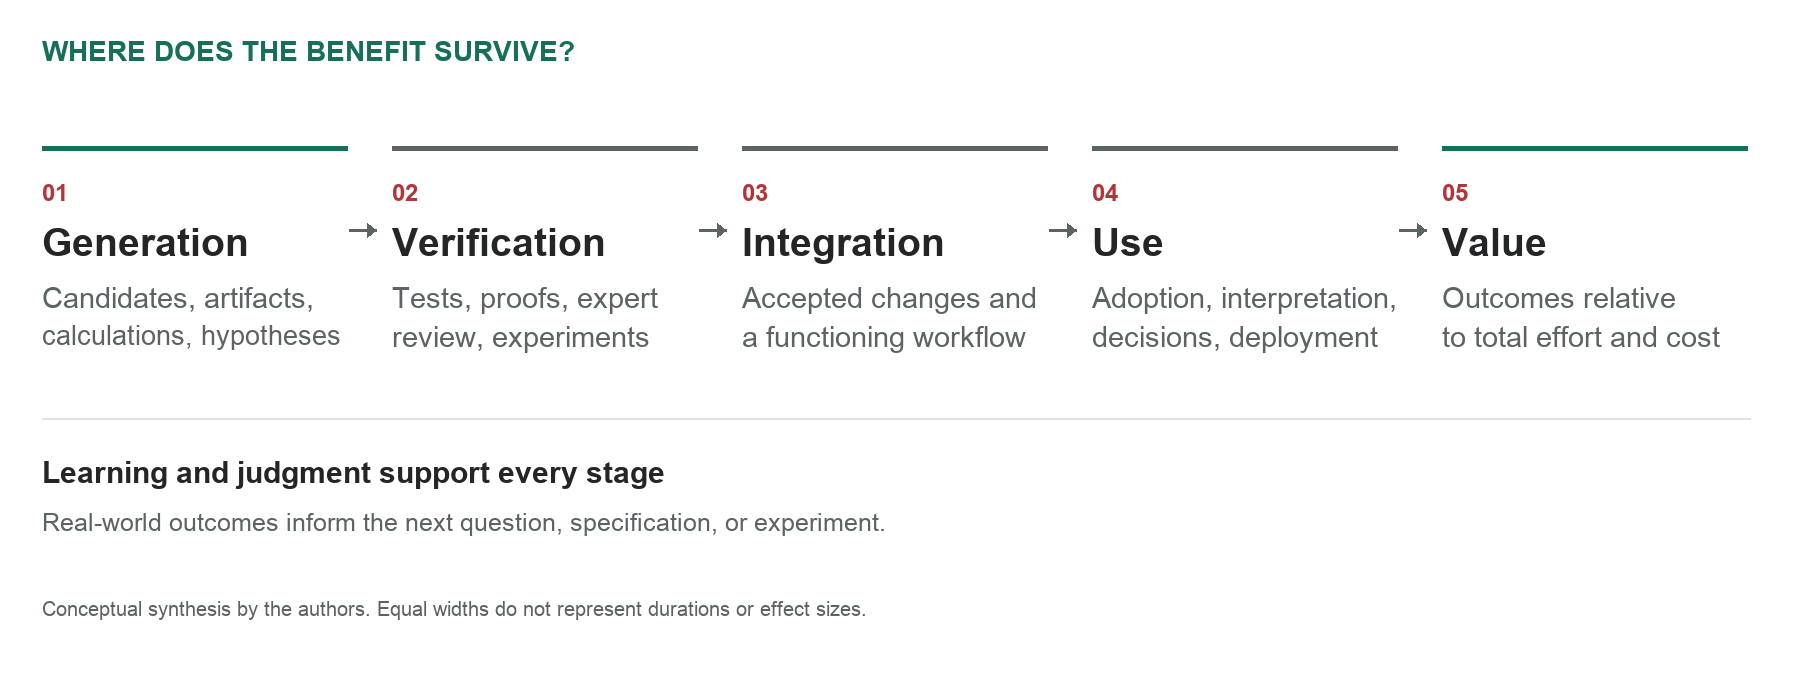
\includegraphics[width=\textwidth]{../site/assets/evidence-pathway.png}\end{figure}



\emph{Figure 1. Evaluation pathway for AI-assisted intellectual work. The stages are conceptual; their equal visual widths do not represent equal durations or estimated effects. Source: authors' synthesis.}


The framework suggests five questions for a particular deployment:


\begin{enumerate}
\item What becomes possible or faster, and relative to which realistic alternative?

\item What evidence makes the result acceptable, and what does verification cost?

\item Can the surrounding workflow integrate the additional output?

\item Is the accepted output used, and does it improve a consequential outcome?

\item What happens to the knowledge and judgment required for the next round of work?
\end{enumerate}

A deployment can succeed without full autonomy. It can also be valuable without producing a large employment effect. Conversely, broad adoption, strong benchmark scores, and enthusiastic user reports remain insufficient to establish the complete value pathway.


The evidence is strongest for specific task and workflow benefits, increasingly informative about downstream engineering constraints, and still heterogeneous on learning and labor effects. Scientific benefits range from well-established specialized predictions to emerging agent workflows with very different degrees of validation. The largest opportunity may include work previously regarded as too complex or expensive to pursue, but its value must still be established through credible results and relevant outcomes.


Our answer to "Does AI Help?" is therefore \textbf{yes in demonstrated settings, no in some tested settings, and unresolved in many others}. AI already helps people produce, search, calculate and explore; it has also measurably slowed expert work, weakened some learning or comprehension outcomes, and imposed costs on reviewers and institutions. Gains and losses can coexist in the same intervention. This collection does not establish whether positive or negative net effects predominate across intellectual work: the outcomes and populations are too different, and selection is not exhaustive. The next research priority is measuring those relationships over time, rather than extrapolating one task's percentage to an entire institution.



\section*{12. Review method, authorship, and release policy}\phantomsection\addcontentsline{toc}{section}{12. Review method, authorship, and release policy}

\subsection*{Scope and selection}\phantomsection\addcontentsline{toc}{subsection}{Scope and selection}
This is a living critical narrative review with an accompanying evidence map. It concentrates on 2023-2026 research while retaining selected earlier foundations. The focus is intellectual work: study, programming, engineering, scientific investigation, and related organizational outcomes. Specialized AI is included where it clarifies a mechanism or provides a credible scientific comparator; findings about specialized models are not automatically attributed to general-purpose LLMs.


The initial collection was supplied and developed over time, then supplemented through primary-source searches of arXiv, journal and publisher sites, research organizations, and selected expert analyses. Searches were organized around productivity experiments, agentic engineering, learning and transfer, AI-supported science, business outcomes, and labor transitions. This release does not claim PRISMA compliance, exhaustive coverage, a preregistered search strategy, or a pooled meta-analytic effect. Coverage is weighted toward English-language sources and the settings in which current evidence is most visible.



\subsection*{Verification and appraisal}\phantomsection\addcontentsline{toc}{subsection}{Verification and appraisal}
The targeted pre-publication search for companion reviews is documented in the \href{https://does-ai-help.github.io/downloads/does-ai-help-related-reviews-2026.10.14.md}{search and reading log}. It adds complementary syntheses without claiming exhaustive coverage or counting their constituent studies as independent new evidence.


Every database record distinguishes \textbf{content-checked}, \textbf{identity-checked}, and \textbf{candidate} status. Content checking records the inspected scope: in some cases a full paper or methods section; in others an abstract or an official summary. Identity checking establishes bibliographic correspondence, not the truth of findings. Candidate records preserve incomplete access or unresolved identification without treating the source as verified evidence. A working link alone does not satisfy result verification.


Core annotations contain an original short summary and limitations. Supporting records have bibliographic and topical descriptions but do not assert unappraised findings. Method, publication status, and relevance are distinct fields. An arXiv DOI identifies a preprint and does not establish peer review. Multiple pages or versions of a work are retained as linked reference records where appropriate, but are not counted as independent replications. The exclusions log records rejected inherited links.


We prefer primary reports for empirical claims. Vendor research and expert essays remain useful when their evidentiary role and interests are explicit. Paywalls and access failures are reported rather than bypassed. Numeric claims are tied to source versions, populations, outcomes, and denominators. Negative or null results receive the same attention as positive findings; statistical insignificance is not automatically evidence of equivalence.


A separate \href{https://does-ai-help.github.io/downloads/does-ai-help-balance-review-2026.10.14.md}{balance self-review and source-admission log} documents evidentiary balance. It distinguishes demonstrated harm, imprecise or null effects, mixed outcomes, forecasts, and community refusal. Equal evidentiary standards do not require equal numbers of positive and negative paragraphs. We do not infer an overall verdict by counting favorable sources, treating duplicate coverage as replication, or treating community opposition as a measured causal effect. Both AI authorship and the human author's business affiliation warrant scrutiny, not a presumption that this review is neutral by construction.


For selected sources that automated CI cannot reliably retrieve or identify, we use a separate \href{https://does-ai-help.github.io/downloads/does-ai-help-browser-verification-guide-2026.10.14.md}{local Chrome verification channel}. The \href{https://does-ai-help.github.io/downloads/does-ai-help-browser-verification-2026.10.14.json}{browser ledger} records the AI-assisted reviewer, observed metadata, exact reading scope and access limits. It is refreshed for each monthly release; previous observations are preserved. A browser confirmation can establish an otherwise unresolved citation, but cannot override an identifier conflict, certify a scientific claim or imply access to subscription full text.


Chang and Huang's journal paper offers survey-based evidence about AI reliance and perceived development performance; only its public preview and snippets were inspected. CNBC's employment account is secondary reporting, not an independent causal study. These reading and methodological limits constrain their evidentiary weight. [\hyperlink{ref-candidate-sciencedirect-2026}{118}, \hyperlink{ref-candidate-cnbc-2026}{119}]


Document inspection includes supplied PDFs matched to their online source versions. Filenames, checksums and exact reading scopes are recorded without redistributing third-party PDFs. The \href{https://does-ai-help.github.io/downloads/does-ai-help-document-followup-2026.10.14.md}{document inspection log} documents title/version differences, assistance-design boundaries and reporting questions for the chess-training, AI Skill Threat and agent-study materials. The Financial Times source is an unappraised candidate because full-text access was unavailable. This access limit is not evidence for or against the article's claims.


Greg Wilson's methodological discussion is a useful companion for readers evaluating common overclaims in AI-assisted coding. The more general lesson is to inspect study design and outcome validity before accepting a headline about productivity. [\hyperlink{ref-wilson2026}{120}]


The CoSLR study supplies a directly relevant caution for AI-assisted evidence synthesis: mandatory checkpoints did not ensure that participants intended to verify generated reports. Its short, survey-based evaluation does not measure actual review accuracy, but motivates explicit citation checks and substantive editorial scrutiny here. Our verification scripts establish bibliographic correspondence, not whether every interpretation is sound. [\hyperlink{ref-coslr2026}{121}]



\subsection*{Authorship and responsibility}\phantomsection\addcontentsline{toc}{subsection}{Authorship and responsibility}
\textbf{GPT 6.1 is credited as the lead AI author}, responsible for organizing the literature, appraising the inspected evidence, developing the synthesis, drafting the article, and preparing the publication materials. \textbf{Witold Bołt is credited as co-author}, responsible for initiating the topic, providing initial links and viewpoints, framing the question, directing the conceptual scope, and initiating this review in its present form.


The AI byline identifies the production method; it does not imply human experience, independent fieldwork, or accountability equivalent to a human researcher. This initial release is an AI-authored review, not a peer-reviewed research publication. Human co-authorship does not by itself assert that every bibliographic record has received a separate human audit. Corrections and changes in source status are part of the release process.


\textbf{Author note.} Witold Bołt, PhD, is Vice-President of \href{https://jit.team}{Jit Team}, a software consulting company. Readers interested in discussing this review or its practical implications may contact \href{mailto:Witold.Bolt@jit.team}{Witold.Bolt@jit.team}, visit Jit Team, or connect through \href{https://www.linkedin.com/in/witoldbolt/}{LinkedIn}. This professional affiliation is disclosed for transparency; it is not evidence for the review's conclusions or an endorsement of any cited product.


\textbf{Reuse and contributions.} The original review and annotations are freely reusable, including commercially, under \href{https://creativecommons.org/licenses/by/4.0/}{Creative Commons Attribution 4.0 International}. Credit GPT 6.1 and Witold Bołt, identify the release, link the license, and indicate changes. Third-party publications retain their own rights. We welcome source suggestions, corrections, and alternative interpretations through \href{https://github.com/does-ai-help/does-ai-help.github.io/issues/new/choose}{GitHub issues} and \href{https://github.com/does-ai-help/does-ai-help.github.io/pulls}{pull requests}; the \href{https://does-ai-help.github.io/downloads/does-ai-help-contributing-2026.10.14.md}{contribution guide} describes the evidence required. Suggestions will be reviewed for monthly releases; submission does not guarantee inclusion.



\subsection*{Monthly maintenance}\phantomsection\addcontentsline{toc}{subsection}{Monthly maintenance}
Each monthly release will preserve its cutoff, source database, article, PDF, changelog, and checksums. New evidence may strengthen or weaken a conclusion, introduce a new mechanism, or simply correct a citation. Updates should prioritize replications, credible interventions, longer-run outcomes, independent datasets, revisions of important working papers, and corrections or retractions. A release should not be generated merely by appending favorable announcements.


The accompanying repository provides machine-readable citation exports, an evidence schema, a reproducible site/PDF build, and a release checklist. Automated link checks support maintenance, while substantive admission and interpretation remain editorial decisions. Stable identifiers connect sources across versions; immutable releases distinguish the historical evidence from the current article.



\section*{Selected references}\phantomsection\addcontentsline{toc}{section}{Selected references}
The references cited in this article follow below. The complete searchable evidence map and downloadable citation files include a broader supporting collection, with verification scope recorded for each entry.


{\small\setlength{\parskip}{0pt}\begin{description}[leftmargin=2em,labelwidth=1.5em,itemsep=1pt,parsep=0pt]
\item[1.] \hypertarget{ref-oecdproductivity2025}{} Flavio Calvino; Jelmer Reijerink; Lea Samek. 2025. \textit{The effects of generative AI on productivity, innovation and entrepreneurship}. organization working paper. \url{https://www.oecd.org/en/publications/the-effects-of-generative-ai-on-productivity-innovation-and-entrepreneurship\_b21df222-en.html}.

\item[2.] \hypertarget{ref-iloreview2026}{} Rossana Merola; Ekkehard Ernst; Daniel Samaan; Maria del Rio-Chanona; Ole Teutloff. 2026. \textit{The impact of GenAI on jobs, productivity and work organization: a review of the empirical evidence}. organization report. \url{https://www.ilo.org/publications/impact-genai-jobs-productivity-and-work-organization-review-empirical}.

\item[3.] \hypertarget{ref-aiindex2026}{} AI Index Stanford Institute for Human-Centered Artificial Intelligence. 2026. \textit{The 2026 AI Index Report}. organization report. \url{https://hai.stanford.edu/ai-index/2026-ai-index-report}.

\item[4.] \hypertarget{ref-ref-59e035c44a}{} Amr Mohamed; Maram Assi; Mariam Guizani. 2025. \textit{The Impact of LLM-Assistants on Software Developer Productivity: A Systematic Review and Mapping Study}. preprint. \url{https://arxiv.org/abs/2507.03156}.

\item[5.] \hypertarget{ref-wittig2026}{} Annemarie Wittig; Alina Mailach; Norbert Siegmund. 2026. \textit{Fragmented Markers, Mixed Results: A Systematic Review of AI Coding Assistants and Developer Productivity}. peer reviewed conference. \url{https://conf.researchr.org/details/ase-2026/ase-2026-research-track/56/Fragmented-Markers-Mixed-Results-A-Systematic-Review-of-AI-Coding-Assistants-and-De}.

\item[6.] \hypertarget{ref-maier2026}{} Sebastian Maier; Moritz Gunzenhäuser; Jonas Schweisthal; Manuel Schneider; Stefan Feuerriegel. 2026. \textit{A meta-analysis of the effect of generative AI on productivity and learning in programming}. preprint. \url{https://arxiv.org/abs/2605.04779}.

\item[7.] \hypertarget{ref-oecdeducation2026}{} OECD. 2026. \textit{OECD Digital Education Outlook 2026: Exploring Effective Uses of Generative AI in Education}. organization report. \url{https://www.oecd.org/en/publications/oecd-digital-education-outlook-2026\_062a7394-en.html}.

\item[8.] \hypertarget{ref-ref-e71e370e4c}{} Said Elnaffar; Farzad Rashidi; Abedallah Zaid Abualkishik. 2025. \textit{Teaching with AI: A Systematic Review of Chatbots, Generative Tools, and Tutoring Systems in Programming Education}. preprint. \url{https://arxiv.org/abs/2510.03884}.

\item[9.] \hypertarget{ref-agenticsurvey2025}{} Jiaqi Wei; Yuejin Yang; Xiang Zhang; et al. 2025. \textit{From AI for Science to Agentic Science: A Survey on Autonomous Scientific Discovery}. preprint. \url{https://arxiv.org/abs/2508.14111v2}.

\item[10.] \hypertarget{ref-alphafold2021}{} John Jumper; Richard Evans; Alexander Pritzel; et al. 2021. \textit{Highly accurate protein structure prediction with AlphaFold}. peer reviewed. \url{https://www.nature.com/articles/s41586-021-03819-2}.

\item[11.] \hypertarget{ref-space2021}{} Nicole Forsgren; Margaret-Anne Storey; Chandra Maddila; et al. 2021. \textit{The SPACE of Developer Productivity: There's More to It than You Think}. research framework. \url{https://queue.acm.org/detail.cfm?id=3454124}.

\item[12.] \hypertarget{ref-noy2023}{} Shakked Noy; Whitney Zhang. 2023. \textit{Experimental evidence on the productivity effects of generative artificial intelligence}. peer reviewed. \url{https://doi.org/10.1126/science.adh2586}.

\item[13.] \hypertarget{ref-peng2023}{} Sida Peng; Eirini Kalliamvakou; Peter Cihon; Mert Demirer. 2023. \textit{The Impact of AI on Developer Productivity: Evidence from GitHub Copilot}. preprint. \url{https://arxiv.org/abs/2302.06590}.

\item[14.] \hypertarget{ref-dellacqua2023}{} Fabrizio Dell'Acqua; Edward McFowland III; Ethan Mollick; et al. 2023. \textit{Navigating the Jagged Technological Frontier: Field Experimental Evidence of the Effects of Artificial Intelligence on Knowledge Worker Productivity and Quality}. author manuscript. Study first circulated in 2023; linked manuscript is a 2026 revision. \url{https://www.hbs.edu/ris/Publication\%20Files/dell-acqua-et-al-2026-navigating-the-jagged-technological-frontier\_5c589c8c-fbb5-458f-b285-c944746cd717.pdf}.

\item[15.] \hypertarget{ref-funsearch2023}{} Bernardino Romera-Paredes; Mohammadamin Barekatain; Alexander Novikov; et al. 2023. \textit{Mathematical discoveries from program search with large language models}. peer reviewed. Published online in December 2023; Nature volume 625 is dated 2024. \url{https://www.nature.com/articles/s41586-023-06924-6}.

\item[16.] \hypertarget{ref-paradis2024}{} Elise Paradis; Kate Grey; Quinn Madison; et al. 2024. \textit{How much does AI impact development speed? An enterprise-based randomized controlled trial}. preprint. \url{https://arxiv.org/abs/2410.12944}.

\item[17.] \hypertarget{ref-cui2025}{} Zheyuan (Kevin) Cui; Mert Demirer; Sonia Jaffe; et al. 2025. \textit{The Effects of Generative AI on High-Skilled Work: Evidence from Three Field Experiments with Software Developers}. research publication. \url{https://www.microsoft.com/en-us/research/publication/the-effects-of-generative-ai-on-high-skilled-work-evidence-from-three-field-experiments-with-software-developers}.

\item[18.] \hypertarget{ref-brynjolfsson2025}{} Erik Brynjolfsson; Danielle Li; Lindsey Raymond. 2025. \textit{Generative AI at Work}. peer reviewed. \url{https://academic.oup.com/qje/article/140/2/889/7990658}.

\item[19.] \hypertarget{ref-dora2024}{} DORA. 2024. \textit{DORA | Accelerate State of DevOps Report 2024}. organization report. \url{https://dora.dev/research/2024/dora-report}.

\item[20.] \hypertarget{ref-messeri2024}{} Lisa Messeri; M. J. Crockett. 2024. \textit{Artificial intelligence and illusions of understanding in scientific research}. peer reviewed perspective. \url{https://www.nature.com/articles/s41586-024-07146-0}.

\item[21.] \hypertarget{ref-metr2025}{} Joel Becker; Nate Rush; Elizabeth Barnes; David Rein. 2025. \textit{Measuring the Impact of Early-2025 AI on Experienced Open-Source Developer Productivity}. preprint. \url{https://arxiv.org/abs/2507.09089}.

\item[22.] \hypertarget{ref-bastani2025}{} Hamsa Bastani; Osbert Bastani; Alp Sungu; et al. 2025. \textit{Generative AI without guardrails can harm learning}. peer reviewed. \url{https://doi.org/10.1073/pnas.2422633122}.

\item[23.] \hypertarget{ref-demirer2026}{} Mert Demirer; Leon Musolff; Liyuan Yang. 2026. \textit{Writing Code vs. Shipping Code: Productivity Effects Across Generations of AI Coding Tools}. working paper. September 2026 revision of the May 2026 working paper. \url{https://www.nber.org/papers/w35275}.

\item[24.] \hypertarget{ref-chenstratton2026}{} Fiona Chen; James Stratton. 2026. \textit{Artificial Intelligence in the Firm: Bottlenecks in Software Production}. working paper. 4 August 2026 revision of the January 2026 working paper. \url{https://fion.ac/jellyfish.pdf}.

\item[25.] \hypertarget{ref-bergh2026}{} Christian Bergh; Benjamin Tag; Alexandra Vassar; Jake Renzella. 2026. \textit{Your Programming Students' Cognition with ChatGPT: Higher Performance, Lower Retention, and Reduced Ownership}. preprint. \url{https://arxiv.org/abs/2609.21194}.

\item[26.] \hypertarget{ref-innovationeval2026}{} David Owen. 2026. \textit{Can AI automate AI R\&D yet?}. organization report. \url{https://epoch.ai/publications/innovationeval}.

\item[27.] \hypertarget{ref-metr2026update}{} Joel Becker; Nate Rush; Tom Cunningham; David Rein; Khalid Mahamud. 2026. \textit{We are Changing our Developer Productivity Experiment Design}. organization report. \url{https://metr.org/blog/2026-02-24-uplift-update}.

\item[28.] \hypertarget{ref-chen2026}{} Valerie Chen; Jasmyn He; Behnjamin Williams; Jason Valentino; Ameet Talwalkar. 2026. \textit{Beyond the Commit: Developer Perspectives on Productivity with AI Coding Assistants}. preprint. \url{https://arxiv.org/abs/2602.03593}.

\item[29.] \hypertarget{ref-afroz2025}{} Sadia Afroz; Zixuan Feng; Tyler Menezes; et al. 2025. \textit{The Fast and Spurious: Developer Productivity with GenAI}. preprint. \url{https://arxiv.org/abs/2510.24265}.

\item[30.] \hypertarget{ref-murphyhill2026}{} Emerson Murphy-Hill; Jenna Butler; Alexandra Savelieva. 2026. \textit{Adoption and Impact of Command-Line AI Coding Agents: A Study of Microsoft's Early 2026 Rollout of Claude Code and GitHub Copilot CLI}. preprint. \url{https://arxiv.org/abs/2607.01418}.

\item[31.] \hypertarget{ref-alphafoldimpact2026}{} Ryan R. Hill; Carolyn Stein. 2026. \textit{How Artificial Intelligence Shapes Science: Evidence from AlphaFold}. working paper. \url{https://www.nber.org/papers/w35143}.

\item[32.] \hypertarget{ref-hemandate2026}{} Hao He; Shyam Agarwal; Yegor Denisov-Blanch; et al. 2026. \textit{AI Writes Faster Than Humans Can Review: A Longitudinal Study of an Enterprise 2x Mandate}. preprint. Version 1. \url{https://arxiv.org/abs/2607.01904v1}.

\item[33.] \hypertarget{ref-faros2026}{} Faros AI. 2026. \textit{AI Impact on Engineering Productivity: 2026 Report Data}. vendor report. \url{https://www.faros.ai/research/ai-acceleration-whiplash}.

\item[34.] \hypertarget{ref-gitclear2025}{} GitClear. 2025. \textit{AI Copilot Code Quality: 2025 Look Back at 12 Months of Data}. vendor report. \url{https://www.gitclear.com/ai\_assistant\_code\_quality\_2025\_research}.

\item[35.] \hypertarget{ref-dora2025}{} Derek DeBellis; Kevin Storer; Nathen Harvey; et al. 2025. \textit{DORA 2025 State of AI-assisted Software Development Report}. organization report. \url{https://research.google/pubs/dora-2025-state-of-ai-assisted-software-development-report}.

\item[36.] \hypertarget{ref-doratensions2026}{} DORA. 2026. \textit{DORA | Balancing AI tensions: Moving from AI adoption to effective SDLC use}. organization analysis. \url{https://dora.dev/insights/balancing-ai-tensions}.

\item[37.] \hypertarget{ref-hamza2026}{} Muhammad Hamza; Dominik Siemon; Wardah Naeem Awan. 2026. \textit{Does Working with AI Agents Change How Developers Code, Test, and Review?}. peer reviewed conference. Published ESEM 2026 version; related SSRN preprints are versions of the same study. \url{https://drops.dagstuhl.de/entities/document/10.4230/LIPIcs.ESEM.2026.67}.

\item[38.] \hypertarget{ref-cotroneo2025}{} Domenico Cotroneo; Cristina Improta; Pietro Liguori. 2025. \textit{Human-Written vs. AI-Generated Code: A Large-Scale Study of Defects, Vulnerabilities, and Complexity}. preprint. \url{https://arxiv.org/abs/2508.21634}.

\item[39.] \hypertarget{ref-sabra2025}{} Abbas Sabra; Olivier Schmitt; Joseph Tyler. 2025. \textit{Assessing the Quality and Security of AI-Generated Code: A Quantitative Analysis}. preprint. \url{https://arxiv.org/abs/2508.14727}.

\item[40.] \hypertarget{ref-tran2026}{} Michael Tran; Fred Lewis; Kun Yang; et al. 2026. \textit{Characterizing the Quality Profile of AI-Generated C++ in Production}. preprint. \url{https://arxiv.org/abs/2608.06640}.

\item[41.] \hypertarget{ref-sweci2026}{} Jialong Chen; Xander Xu; Hu Wei; Chuan Chen; Bing Zhao. 2026. \textit{SWE-CI: Evaluating Agent Capabilities in Maintaining Codebases via Continuous Integration}. preprint. \url{https://arxiv.org/abs/2603.03823}.

\item[42.] \hypertarget{ref-coverage2026}{} Atish Kumar Dipongkor; Talank Baral; Wing Lam; Kevin Moran. 2026. \textit{Test Coverage Analysis of Agentic Pull Requests}. preprint. \url{https://arxiv.org/abs/2607.18057}.

\item[43.] \hypertarget{ref-iac2026}{} Benjamin Agyekum; Fabio Santos. 2026. \textit{Does Fixing Break Security? An Empirical Study of Security Degradation in Iterative LLM-Driven Infrastructure-as-Code Repair}. preprint. \url{https://arxiv.org/abs/2608.13404}.

\item[44.] \hypertarget{ref-vero2026}{} Zhe Ye; Hantao Lou; Yuechun Sun; et al. 2026. \textit{Vero: Can AI Agents Build Formally Verified Software Repositories?}. preprint. \url{https://arxiv.org/abs/2608.13522}.

\item[45.] \hypertarget{ref-qemupolicy2026}{} QEMU project. 2025. \textit{Code provenance}. project documentation. \url{https://www.qemu.org/docs/master/devel/code-provenance.html}.

\item[46.] \hypertarget{ref-gimppolicy2026}{} GIMP team. 2026. \textit{Giving or obtaining developer access in Gitlab}. project documentation. \url{https://developer.gimp.org/core/maintainer/giving-developer-right/}.

\item[47.] \hypertarget{ref-redoxpolicy2026}{} Redox OS contributors. 2026. \textit{Contributing to Redox}. project documentation. \url{https://github.com/redox-os/redox/blob/master/CONTRIBUTING.md}.

\item[48.] \hypertarget{ref-zigpolicy2026}{} Zig project. 2025. \textit{Code of Conduct}. project documentation. \url{https://ziglang.org/code-of-conduct/}.

\item[49.] \hypertarget{ref-netbsdpolicy2024}{} NetBSD project. 2024. \textit{NetBSD Commit Guidelines}. project documentation. \url{https://www.netbsd.org/developers/commit-guidelines.html}.

\item[50.] \hypertarget{ref-linuxgenerated2026}{} Linux kernel development community. 2026. \textit{Kernel Guidelines for Tool-Generated Content}. project documentation. \url{https://docs.kernel.org/process/generated-content.html}.

\item[51.] \hypertarget{ref-linuxassistants2026}{} Linux kernel development community. 2026. \textit{AI Coding Assistants}. project documentation. \url{https://docs.kernel.org/process/coding-assistants.html}.

\item[52.] \hypertarget{ref-torvaldsassoc2026}{} Michael Larabel. 2026. \textit{Linus Torvalds "Did What I Preach", Used AI To Make Code Decipherable \& Uncovered More Bugs}. journalism. \url{https://www.phoronix.com/news/Linus-Torvalds-Assoc-Array}.

\item[53.] \hypertarget{ref-asahipolicy2026}{} Asahi Linux project. 2026. \textit{Generative AI (LLM) Policy}. project documentation. \url{https://asahilinux.org/llm-policy/}.

\item[54.] \hypertarget{ref-gravityabout2026}{} Gravity Linux contributors. 2026. \textit{About - Gravity Linux}. project documentation. \url{https://gravitylinux.org/about/}.

\item[55.] \hypertarget{ref-gravitypolicy2026}{} Gravity Linux contributors. 2026. \textit{LLM Use and Clean-Room Policy}. project documentation. \url{https://gravitylinux.org/policies/llm/}.

\item[56.] \hypertarget{ref-ghosttypolicy2026}{} Ghostty project. 2026. \textit{AI Usage Policy}. project documentation. \url{https://github.com/ghostty-org/ghostty/blob/00c33eaf72af6c9b93d9fd8d54b6f7086612a95b/AI\_POLICY.md}.

\item[57.] \hypertarget{ref-ghosttycontribution2026}{} Ghostty project. 2026. \textit{Contributing to Ghostty}. project documentation. \url{https://github.com/ghostty-org/ghostty/blob/22f9233a0f7b85747483ce713411c67be4643d8f/CONTRIBUTING.md}.

\item[58.] \hypertarget{ref-horapolicies2026}{} Andre Hora; Romain Robbes; Stefano Zacchiroli. 2026. \textit{"We Permit the Use of AI, but [...]": The Landscape of AI Policies in Popular Open Source Projects}. preprint. Expanded version of the earlier 118-policy study; not an independent replication. Under review, not an accepted journal paper. \url{https://arxiv.org/abs/2609.07542}.

\item[59.] \hypertarget{ref-shen2026}{} Judy Hanwen Shen; Alex Tamkin. 2026. \textit{How AI Impacts Skill Formation}. preprint. \url{https://arxiv.org/abs/2601.20245}.

\item[60.] \hypertarget{ref-ref-283d4e8368}{} Stefanos Poulidis; Hamsa Bastani; Osbert Bastani. 2025. \textit{Self-Regulated AI Use Hinders Long-Term Learning}. working paper. \url{https://papers.ssrn.com/sol3/papers.cfm?abstract\_id=5604932}.

\item[61.] \hypertarget{ref-ownership2026}{} Alberto Martin-Lopez; Rosalia Tufano; Emanuela Guglielmi; et al. 2026. \textit{More Code, Less Understanding? On the Impact of AI Assistants on Developers' Productivity and Code Ownership}. peer reviewed. \url{https://personal.us.es/amarlop/wp-content/uploads/2026/03/More-Code-Less-Understanding-On-the-Impact-of-AI-Assistants-on-Developers-Productivity-and-Code-Ownership.pdf}.

\item[62.] \hypertarget{ref-lepp2026}{} Marina Lepp. 2026. \textit{Patterns of Learner-AI Interaction and Academic Performance in an Object-Oriented Programming Course}. preprint. \url{https://arxiv.org/abs/2607.24755}.

\item[63.] \hypertarget{ref-wang2026}{} Shihao Wang. 2026. \textit{A Risk-Adaptive and Evidence-Constrained Framework for Generative AI Feedback in Programming Education}. preprint. \url{https://arxiv.org/abs/2609.29874}.

\item[64.] \hypertarget{ref-wulearning2026}{} Xinning Wu; Pei Zhu; Jinliang Zhang; Mengwei Yin; Yingxi Wang. 2026. \textit{ChatGPT's impact on student learning outcomes: a meta-analysis of 35 experimental studies}. peer reviewed. \url{https://www.nature.com/articles/s41599-026-07019-z}.

\item[65.] \hypertarget{ref-boolzen2026}{} Chiara Boolzen; Jochen Kuhn; Salome Flegr; et al. 2026. \textit{Evidence of impact and interpretational limits of generative AI in STEM education: a systematic review and meta-analysis on cognitive learning outcomes}. peer reviewed. \url{https://link.springer.com/article/10.1007/s10462-026-11665-9}.

\item[66.] \hypertarget{ref-llamalima2026}{} Anselm Strohmaier; Samira Bödefeld; Oliver Straser; Frank Reinhold. 2026. \textit{LLAMA LIMA: A Living Meta-Analysis on the Effects of Generative AI on Learning Mathematics}. preprint. Version 5, 11 September 2026. \url{https://arxiv.org/abs/2601.18685v5}.

\item[67.] \hypertarget{ref-vella2026}{} Annie Vella; Kelly Blincoe. 2026. \textit{The Impact of AI Coding Assistants on Software Engineering: A Longitudinal Study}. preprint. \url{https://arxiv.org/abs/2605.23135}.

\item[68.] \hypertarget{ref-brand2026}{} Charlotte Brandebusemeyer; Daniela Gasser; Tobias Schimmer; Bert Arnrich. 2026. \textit{Beyond Productivity: Measuring Developers' Cognitive Load During GenAI-Supported Software Development}. preprint. \url{https://arxiv.org/abs/2609.37645}.

\item[69.] \hypertarget{ref-ref-47ac0a3015}{} Catherine M. Hicks; Carol S. Lee; Kristen L. Foster-Marks. 2025. \textit{AI Skill Threat: How the Structure of Developers' Beliefs about Software Development Ability Impacts Their Psychological Resilience During Rapid Technology Shift}. preprint. \url{https://osf.io/preprints/psyarxiv/2gej5\_v2}.

\item[70.] \hypertarget{ref-era2026}{} Eser Aygün; Anastasiya Belyaeva; Gheorghe Comanici; et al. 2026. \textit{An AI system to help scientists write expert-level empirical software}. peer reviewed. \url{https://www.nature.com/articles/s41586-026-10658-6}.

\item[71.] \hypertarget{ref-coscientist2026}{} Juraj Gottweis; Wei-Hung Weng; Alexander Daryin; et al. 2026. \textit{Accelerating scientific discovery with Co-Scientist}. peer reviewed. \url{https://www.nature.com/articles/s41586-026-10644-y}.

\item[72.] \hypertarget{ref-robin2026}{} Ali E. Ghareeb; Benjamin Chang; Ludovico Mitchener; et al. 2026. \textit{A multi-agent system for automating scientific discovery}. peer reviewed. \url{https://www.nature.com/articles/s41586-026-10652-y}.

\item[73.] \hypertarget{ref-aiscientist2026}{} Chris Lu; Cong Lu; Robert Tjarko Lange; et al. 2026. \textit{Towards end-to-end automation of AI research}. peer reviewed. \url{https://www.nature.com/articles/s41586-026-10265-5}.

\item[74.] \hypertarget{ref-alphaproof2025}{} Thomas Hubert; Rishi Mehta; Laurent Sartran; et al. 2026. \textit{Olympiad-level formal mathematical reasoning with reinforcement learning}. peer reviewed. \url{https://www.nature.com/articles/s41586-025-09833-y}.

\item[75.] \hypertarget{ref-alphaevolve2025}{} Alexander Novikov; Ngân Vũ; Marvin Eisenberger; et al. 2025. \textit{AlphaEvolve: A coding agent for scientific and algorithmic discovery}. preprint. \url{https://arxiv.org/abs/2506.13131}.

\item[76.] \hypertarget{ref-discorl2025}{} Junhyuk Oh; Gregory Farquhar; Iurii Kemaev; et al. 2025. \textit{Discovering state-of-the-art reinforcement learning algorithms}. peer reviewed. \url{https://www.nature.com/articles/s41586-025-09761-x}.

\item[77.] \hypertarget{ref-schwartz2026}{} Matthew Schwartz. 2026. \textit{Claude-shaped science}. vendor hosted essay. \url{https://www.anthropic.com/research/claude-shaped-science}.

\item[78.] \hypertarget{ref-hao2026}{} Qianyue Hao; Fengli Xu; Yong Li; James Evans. 2026. \textit{Artificial intelligence tools expand scientists’ impact but contract science’s focus}. peer reviewed. \url{https://www.nature.com/articles/s41586-025-09922-y}.

\item[79.] \hypertarget{ref-leiden2026}{} Jarod Alper; Michael Barany; Alain Chavarri Villarello; et al. 2026. \textit{Leiden Declaration on Artificial Intelligence and Mathematics}. public statement. Declaration DOI: 10.5281/zenodo.20302944. The later arXiv manifestation is the same declaration. \url{https://leidendeclaration.ai/}.

\item[80.] \hypertarget{ref-taoicm2026}{} Terence Tao. 2026. \textit{Mathematics in the age of AI}. preprint. \url{https://arxiv.org/abs/2608.16753v1}.

\item[81.] \hypertarget{ref-taomath2026}{} Terence Tao. 2026. \textit{Math 2.0}. lecture slides. \url{https://teorth.github.io/tao-web/slides/math-2-0-caltech-2026.pdf}.

\item[82.] \hypertarget{ref-klowdentao2026}{} Tanya Klowden; Terence Tao. 2026. \textit{Mathematical methods and human thought in the age of AI}. preprint. \url{https://arxiv.org/abs/2603.26524v1}.

\item[83.] \hypertarget{ref-mathmisalignment2026}{} Terence Tao et al. 2026. \textit{A Severe Misalignment of AI in Mathematics}. public statement. \url{https://mathandai.org/}.

\item[84.] \hypertarget{ref-ahm2026}{} Association for Human Mathematics Communications Working Group. 2026. \textit{AHM Statement on OpenAI's October 6 Release of Mathematical Documents}. public statement. \url{https://www.ahmath.org/statements}.

\item[85.] \hypertarget{ref-taoliving2026}{} Terence Tao. 2026. \textit{Terence Tao on AI in mathematics (and beyond)}. living essay. \url{https://teorth.github.io/tao-web/ai-views.html}.

\item[86.] \hypertarget{ref-openainavier2026}{} OpenAI. 2026. \textit{On the Navier-Stokes Millennium Prize Problem}. organization announcement. \url{https://openai.com/index/navier-stokes-solution/}.

\item[87.] \hypertarget{ref-openainavierpaper2026}{} OpenAI. 2026. \textit{Finite time blowup for Navier-Stokes}. technical manuscript. \url{https://cdn.openai.com/pdf/32d9f210-8b73-45e0-91bc-82a30aef8a9a/navier-stokes.pdf}.

\item[88.] \hypertarget{ref-openainaviercode2026}{} OpenAI. 2026. \textit{Finite time blowup for Navier-Stokes and Euler equations}. research software. \url{https://github.com/openai/NavierStokesAndEuler/tree/f9e8bc5b38b6e212696e8a30e3e91517af887bbd}.

\item[89.] \hypertarget{ref-claynavier2026}{} Clay Mathematics Institute. 2026. \textit{Navier-Stokes Announcement}. organization announcement. \url{https://www.claymath.org/news/navier-stokes-announcement/}.

\item[90.] \hypertarget{ref-naviertranslation2026}{} Alexander Bastounis; Fabian Circelli; Anders C. Hansen. 2026. \textit{Navier-Stokes lost in translation: Why Lean verification of AI autoformalisation does not guarantee correct natural language proofs}. preprint. \url{https://arxiv.org/abs/2610.08144v1}.

\item[91.] \hypertarget{ref-hales2026}{} Thomas Hales. 2026. \textit{What mathematicians should know about the Lean Theorem Prover: questions of reliability and AI}. expert essay. \url{https://terrytao.wordpress.com/2026/10/09/what-mathematicians-should-know-about-the-lean-theorem-proverquestions-of-reliability-and-ai/}.

\item[92.] \hypertarget{ref-demourakernel2026}{} Leonardo de Moura. 2026. \textit{Postmortem for the Kernel Soundness Bug Hunt}. expert technical report. \url{https://leodemoura.github.io/blog/2026-8-24-postmortem-for-the-kernel-soundness-bug-hunt/}.

\item[93.] \hypertarget{ref-dgm2025}{} Jenny Zhang; Shengran Hu; Cong Lu; Robert Lange; Jeff Clune. 2025. \textit{Darwin Godel Machine: Open-Ended Evolution of Self-Improving Agents}. preprint. \url{https://arxiv.org/abs/2505.22954}.

\item[94.] \hypertarget{ref-darwinx2026}{} Yifan Zhang; Yutong Dai; Juntao Tan; et al. 2026. \textit{DarwinX: Evolving Agent Harnesses Through Natural Selection}. preprint. \url{https://arxiv.org/abs/2608.07545}.

\item[95.] \hypertarget{ref-interfaces2026}{} Xiangzhe Xu; Hamidreza Saghir; Qianhui Wu; et al. 2026. \textit{The Devil Is in the Interface: Evaluating How Tool Architecture Shapes Coding Agent Behavior}. preprint. \url{https://arxiv.org/abs/2608.11386}.

\item[96.] \hypertarget{ref-researchgym2026}{} Aniketh Garikaparthi; Manasi Patwardhan; Arman Cohan. 2026. \textit{ResearchGym: Evaluating Language Model Agents on Real-World AI Research}. preprint. \url{https://arxiv.org/abs/2602.15112}.

\item[97.] \hypertarget{ref-alignment2026}{} Chen Yueh-Han; Jiaxin Wen; Jan Hendrik Kirchner. 2026. \textit{Automated Researchers Can Mitigate Well-Characterized Alignment Failures}. vendor research report. \url{https://alignment.anthropic.com/2026/automated-alignment-researchers}.

\item[98.] \hypertarget{ref-rdmetrics2026}{} Anthropic. 2026. \textit{Measurements for understanding the pace of AI development inside frontier labs}. vendor report. \url{https://www.anthropic.com/institute/measuring-pace-of-ai-development}.

\item[99.] \hypertarget{ref-ref-fee88585ea}{} KPMG International. 2026. \textit{Growing adoption signals progress as cost visibility and accountability drive AI value, new KPMG Global AI Pulse survey finds}. press release. \url{https://kpmg.com/xx/en/media/press-releases/2026/06/growing-adoption-signals-progress-as-cost-visibility-and-accountability-drive-ai-value.html}.

\item[100.] \hypertarget{ref-kpmgpulseq32026}{} Priya Emmanuel; Benedikt Höck; Simon Benson. 2026. \textit{Global AI Pulse Q3 2026: AI at scale: Accountability, resilience and economics}. industry report. \url{https://assets.kpmg.com/content/dam/kpmgsites/xx/pdf/2026/09/global-ai-pulse.pdf.coredownload.inline.pdf}.

\item[101.] \hypertarget{ref-uber2026}{} Simon Willison. 2026. \textit{Uber Caps Usage of AI Tools Like Claude Code to Manage Costs}. expert blog. \url{https://simonwillison.net/2026/Jun/3/uber-caps-usage}.

\item[102.] \hypertarget{ref-iqbal2026}{} Fazla Iqbal; Muhammad Asif Khan; Oshani Weerakoon; Shola Oyedeji; Jari Porras. 2026. \textit{The Impacts of Artificial Intelligence throughout the Software Development Life-cycle on Sustainability: A Mixed-method Study}. peer reviewed workshop. \url{https://dl.acm.org/doi/10.1145/3786148.3788622}.

\item[103.] \hypertarget{ref-retail2025}{} Lu Fang; Zhe Yuan; Kaifu Zhang; Dante Donati; Miklos Sarvary. 2025. \textit{Generative AI and Sales Productivity: Field Experiments in Online Retail}. preprint. 29 June 2026 revision. \url{https://arxiv.org/abs/2510.12049}.

\item[104.] \hypertarget{ref-babina2026}{} Tania Babina; Alex X. He; Renhao Jiang. 2026. \textit{Canaries in the Gold Mine: Early Productivity Gains from Artificial Intelligence Creating Organization Capital}. working paper. \url{https://www.nber.org/papers/w35684}.

\item[105.] \hypertarget{ref-pragmatic2026}{} Gergely Orosz; Elin Nilsson. 2026. \textit{The impact of AI on software engineers in 2026: key trends. Part 1}. expert newsletter. \url{https://newsletter.pragmaticengineer.com/p/the-impact-of-ai-on-software-engineers-2026}.

\item[106.] \hypertarget{ref-kompella2026}{} Kashyap Kompella. 2026. \textit{The risks of AI overreliance in software engineering}. industry analysis. \url{https://www.techtarget.com/ai/tip/The-risks-of-AI-overreliance-in-software-engineering}.

\item[107.] \hypertarget{ref-gates2026}{} Bill Gates. 2026. \textit{The turbulent AI era is here. The choices we make now are critical.}. expert essay. \url{https://www.gatesnotes.com/work/make-ai-work-for-everyone/reader/a-turbulent-ai-era-and-critical-choices-to-make}.

\item[108.] \hypertarget{ref-mukherjee2026}{} Andy Mukherjee. 2026. \textit{AI Is Eating Software and Investors Have Noticed}. opinion. \url{https://www.advisorperspectives.com/articles/2026/10/08/ai-eating-software-investors-noticed?topic=small-cap}.

\item[109.] \hypertarget{ref-orland2026}{} Kyle Orland. 2026. \textit{AI coding agents generate more code, but not more software}. journalism. \url{https://arstechnica.com/ai/2026/10/ai-coding-agents-generate-more-code-but-not-more-software/}.

\item[110.] \hypertarget{ref-humlum2026}{} Anders Humlum; Emilie Vestergaard. 2025. \textit{Still Waters, Rapid Currents: Early Labor Market Transformation under Generative AI}. working paper. March 2026 revision of the May 2025 working paper. \url{https://www.nber.org/papers/w33777}.

\item[111.] \hypertarget{ref-stanford2025}{} Erik Brynjolfsson; Bharat Chandar; Ruyu Chen. 2025. \textit{Canaries in the Coal Mine? Six Facts about the Recent Employment Effects of Artificial Intelligence - Stanford Digital Economy Lab}. working paper. \url{https://digitaleconomy.stanford.edu/publication/canaries-in-the-coal-mine-six-facts-about-the-recent-employment-effects-of-artificial-intelligence}.

\item[112.] \hypertarget{ref-westby2026}{} Samuel Westby; Alicia Sasser Modestino; Peiran Cheng. 2026. \textit{Generative AI and the Redefinition of Entry-Level Software Work}. working paper. \url{https://www.iza.org/publications/dp/18723/generative-ai-and-the-redefinition-of-entry-level-software-work}.

\item[113.] \hypertarget{ref-ramp2026}{} Ara Kharazian; Lisa Simon; Ryan Stevens. 2026. \textit{A New Look at AI's Impact on Jobs: Firm-Level AI Spending and Workforce Adjustment}. vendor working paper. \url{https://ramp.com/data/ai-jobs-impact/paper}.

\item[114.] \hypertarget{ref-herrengt2026}{} Florian Herrengt. 2026. \textit{AI is removing the middle class of software engineering}. expert blog. \url{https://blog.florianherrengt.com/ai-removing-middle-class-software-engineering.html}.

\item[115.] \hypertarget{ref-herrengtvibe}{} Florian Herrengt. 2025. \textit{The vibe coder's career path is doomed}. expert blog. \url{https://blog.florianherrengt.com/vibe-coder-career-path.html}.

\item[116.] \hypertarget{ref-nscc2026}{} National Student Clearinghouse. 2026. \textit{The Changing Landscape of Postsecondary Education}. organization report. \url{https://www.studentclearinghouse.org/nscblog/changing-landscape-of-postsecondary-education}.

\item[117.] \hypertarget{ref-hesa2026}{} HESA / Jisc. 2026. \textit{UK higher education student numbers fall for second year in a row}. official statistics. \url{https://www.hesa.ac.uk/news/27-01-2026/uk-he-student-numbers-fall-second-year-in-a-row}.

\item[118.] \hypertarget{ref-candidate-sciencedirect-2026}{} Tsung-Sheng Chang; Lan-Gui Huang. 2026. \textit{The impact of generative artificial intelligence on software development performance: a study based on the theory of technology dominance}. peer reviewed. \url{https://www.sciencedirect.com/science/article/abs/pii/S0378720626000066}.

\item[119.] \hypertarget{ref-candidate-cnbc-2026}{} Corynn Winston. 2026. \textit{AI is automating coding. So why are software developer job postings on the rise?}. journalism. \url{https://www.cnbc.com/2026/10/11/ai-software-developer-jobs.html}.

\item[120.] \hypertarget{ref-wilson2026}{} Greg Wilson. 2026. \textit{Twelve Ways to Be Wrong About AI-Assisted Coding}. expert blog. \url{https://third-bit.com/2026/05/20/twelve-ways-to-be-wrong}.

\item[121.] \hypertarget{ref-coslr2026}{} MD Aidul Islam; Malik Abdul Sami; Muhammad Waseem; et al. 2026. \textit{Checkpoints Are Not Enough: Trust Calibration in CoSLR, a Human-AI System for Systematic Literature Reviews}. preprint. \url{https://arxiv.org/abs/2609.22248}.
\end{description}}
